\documentclass[conference]{IEEEtran}
\IEEEoverridecommandlockouts
% The preceding line is only needed to identify funding in the first footnote. If that is unneeded, please comment it out.
\usepackage{cite}
\usepackage{hyperref}
\usepackage{amsmath,amssymb,amsfonts}
\usepackage{algorithmic}
\usepackage{graphicx}
\usepackage{textcomp}
\usepackage{xcolor}
\def\BibTeX{{\rm B\kern-.05em{\sc i\kern-.025em b}\kern-.08em
    T\kern-.1667em\lower.7ex\hbox{E}\kern-.125emX}}
\begin{document}

\title{Face Mask Detection Using Convolutional Neural Network (CNN) : Ensure Safety During COVID- 19 \\}

\author{\IEEEauthorblockN{1\textsuperscript{st} Md. Hasan Imam Shihab}
\IEEEauthorblockA{\textit{dept. of Computer Science and Engineering} \\
\textit{East West University}\\
Dhaka, Bangladesh \\
hasan.shihabimam@gmail.com}
\and

\IEEEauthorblockN{2\textsuperscript{nd} Omair Bin Abdur Rahman}
\IEEEauthorblockA{\textit{dept. of Computer Science and Engineering} \\
\textit{East West University}\\
Dhaka, Bangladesh \\
omairbin.rahman@gmail.com}
\and
\IEEEauthorblockN{3\textsuperscript{rd} Raunaq Tabbassum}
\IEEEauthorblockA{\textit{dept. of Computer Science and Engineering} \\
\textit{East West University}\\
Dhaka, Bangladesh \\
traunok@gmail.com}
\and
\IEEEauthorblockN{4\textsuperscript{th} Razoana Ayshee}
\IEEEauthorblockA{\textit{dept. of Computer Science and Engineering} \\
\textit{East West University}\\
Dhaka, Bangladesh \\
razoanaayshee1@gmail.com}


}

\maketitle

\begin{abstract}
COVID-19 has created the world wide pandemic in recent times. To prevent COVID-19 we have to follow some safety rules, such  as  physical-distancing,  wearing  a  face-mask,  keeping  rooms  well  ventilated,avoiding  crowds,  cleaning  your  hands,  and  coughing  into a bent elbow or tissue .  In  many  cases  people are not following those safety rules. In most of the case the people do not wear any face-mask in a crowded public area and do not maintain social safe distancing, which will increase the infection of COVID-19 among people. This is the reason for which the social safety  related to COVID-19 has becoming very popular topic  among  researchers.  Many  researchers  suggested effective model in order to create social awareness among the people.  Therefore,  this  study  has  been  designed  to established a system which can ensure public safety by detecting a person is wearing face-mask or not in a public place. Finding  out  weather  a  person  is  following  the  safety rules  and  regulation  which  recommended  by  world  health organization  (WHO)  to  prevent  mass  spread  of  coronavirus and  admonish  him  or  her  to  follow  the  rules  and  regulation is  going  to  be  really  helpful  to  prevent  the  spread  of  coronavirus and break the infection chain of COVID-19. For this research we have collected 12,000 image data from kaggle where the images contain person's images with and without mask. Then  we used TensorFlow, Keras and ImageDataGenerator along with Convolutional Neural Network(CNN) in order to build our desired face-mask detection model. This research paper  is  going  to  be  useful  for  saving the people from the infection of COVID-19. Do not following the safety rules in public place is Strictly forbidden  and  this  paper  is  designed  to  make  people  aware about  their duty to the society during COVID-19 pandemic. In previous researches they have also suggested many model to ensure safety during COVID-19 but there are many dimension left to explore on this topic. Every conscious people and authority will be interested in our findings to  make sure the social safety in the crowed public place.
\end{abstract}
\begin{IEEEkeywords}
COVID-19, Face-Mask, TensorFlow, OpenCV, Keras, ImageDataGenerator,  Convolutional Neural Network (CNN), Kaggle data-set, Public Safety.
\end{IEEEkeywords}

\section{Introduction}
COVID-19 is the disease caused by a new type of coronavirus, SARS-COV-2 that can affect upper respiratory tract or lower respiratory tract (windpipe and lungs). COVID-19 has caused 
a worldwide pandemic. For the first time in December 2019, COVID-19 outbreak in China and the outbreak spread quickly as a threat to human physical health around the world. There are some vaccine available against the COVID-19. The World Health Organization (WHO) assume that  a vaccine efficacy of 67\% may be enough to slow the pandemic\cite{VACCINE} but it is impossible to vaccination the whole population at a short period of time. That is why preventive measures are extremely important to reduce the risk of infection in the society. The World Health Organization (WHO) suggested everyone to maintain certain guidelines in order to prevent and control the infection, such as physical distancing, wearing a mask, keeping rooms well ventilated, avoiding crowds, cleaning your hands, and coughing into a bent elbow or tissue\cite{feng2020rational}. It is specially important to wear a mask when you are with people you do not live with because, COVID-19 spreads mainly through respiratory droplets from person to person. Some Researches shows that masks reduce or prevent the spray of people's droplets from reaching others\cite{leung2020respiratory}. The research shows that majority of the COVID positive cases found in crowded and over crowded areas\cite{agarwal2020face}. Therefore, it is important to wear mask in the public place specially, in crowded place like, shopping mall, public transport, supper-shop, etc in order to prevent transmission of the disease\cite{feng2020rational}.
The right way to wear a mask is by adjusting the mask to cover the mouth, nose, and chin\cite{WHO}. The protection from coronavirus will reduce in a great amount if people does not wear mask properly\cite{jiang2021real}. \\

In recent times, many service providers, shops, shopping-mall and organizations ask customer to use the service only if they wear face masks\cite{fang2020transmission}.To ensure the citizen's safety, security guards are arranged in public places to remind people to wear masks but, this measure not only exposes the guards to the air that may contain the virus, but also leads to overcrowding at the entrances due to its inefficiency\cite{jiang2021real}. Therefore, detection on conditions where peoples are wearing face mask or not in the public places have become a valuable and meaningful computer vision task\cite{zhang2021novel}. \\

Computer vision is an interdisciplinary scientific field that involves how computer gain advanced understanding from digital images and videos which include image classification, object detection, image processing, and image recognition. Artificial Intelligence (AI) can be used in many ways for preventing the transmission of COVID-19. In those cases we can use Machine Learning(ML) and Deep learning(DL) algorithms in order to detect face- mask, social distancing etc\cite{agarwal2020unleashing}. We proposed to build a face-mask detection model by using  Convolutional Neural Network (CNN) in this paper. Convolutional Neural Network (CNN)  is a class of Deep Neural Network (DNN) under Deep Learning (DL) which most commonly used in image classification and and recognition. In order to implement this model we use TensorFlow  to build our model and classify the model. TensorFlow has a comprehensive, flexible ecosystem of tools, libraries and community researchers push the state of the art in ML powered applications.
ImageDataGenerator class provides a quick and easy way to augment the images.  We apply ImageDataGenerator on each training image as it is passed to the model. We used OpenCV to high-level understanding from the digital images.Keras is an API designed for human beings. We used Keras to develop our model, layer and test our model. There are no efficient face mask detection applications to 
detect weather the person is wearing face mask or not and this 
increases the demand for an efficient system for detecting 
face masks on people's face in public transport, densely 
populated areas, shopping-malls, and any other crowded areas. This 
project uses Convolutional Neural Network(CNN) with OpenCV, ImageDataGenerator, Keras, and Tensorflow to detect face-masks on people's face.\\
\subsection{Research Aim and Objectives}
Finding out and weather a person is following the safety rules and regulation which recommended by world health organization (WHO) to prevent mass spread of coronavirus and admonish him or her to follow the rules and regulation is going to be really helpful to prevent the spread of corona virus and break the infection chain of COVID-19.\\\\
There  are  some  objectives  which  need  to  be  fulfilled  to achieve the study goal are:\\
-To detect a person is wearing a face-mask or not and maintaining a safe social distance in crawdad and public places.\\
-To create awareness among people about the preventive safety rules of COVID-19.\\
\subsection{Research Question}
To  find  out  a  better  understanding  on  Face Mask Detection in order to prevent corona pandemic,  we  propose  a  research  question,  which  is- How our proposed model with Convolutional Neural Network (CNN) is going to find out peoples face with mask and without mask and contribute to prevent coronvirus's spreading. 
To   find   out   the   answer   of   the   research   question   and step  forward  to  the  aim  we  have  collected  data of human's picture with wearing and without wearing mask and build the face-mask detection model.

\section{Related Work}
Face detection, skeleton detection, sign detection, and pedestrian detection is a most focused task in computer vision in this modern time\cite{benenson2014ten}\cite{fu2010survey}. Normally, most of the works focus on image reconstruction and face recognition for a person's identity verification, moreover face recognition is always a hot-spot in object detection\cite{yadav2020deep}.Guanjun at el \cite{A1} proposed face detection model which performs direct classification on DCFs, compared with the state of the art face detection methods using CNN, which can significantly progress the face detection process efficiency. Also the proposed method can detect small-size faces by using the sliding window strategy on DCFs, where since the performance of these method is greatly affected  by the object proposal quality generated by the object proposal generation method's current state of the art face detection methods based on CNN are still challenging task to detect small sized faces\cite{A1}. Not only face detection for identity but also Because of COVID-19 pandemic face-mask detection technique attracted much attention of researchers and the face-mask detection model has become most essential model during this pandemic\cite{jiang2021real}. \\

There are many researches performed and researchers already build many essential model to detect whether a person is wearing a mask or not. Using hand-crafted and deep learning (YOLOv3 and CNNs) features and (support vector machine) SVM classifiers has been a significant field of research for the detection and recognition of masked faces\cite{A2}. Liu at el \cite{A2} proposed a deep learning detection model YOLOv3 which can work robustly for  multi object detection was used for detecting and also crop all the faces in the novel data-set which contains huge variety of image sizes where the largest size of images is 608x883 and the smallest is 3x4. YOLOv3 was used also to detect and  crops all the videos collected from the public. A model was built to detect face- mask in order to monitor students in the classroom where he or she is wearing a mask or not by using deep Convolutional neural network (CNN)\cite{E1}. In their project they used the ResNet50 deep learning network to check whether the students in the classroom were wearing masks or not.They use deep learning techniques for more accurate
results\cite{E1}. ResNet50 is CNN architecture which was already pre-trained on ImageNet database. K.Nithiyasree at el \cite{E1} capture images by using OpenCV and save those images by using
student names. Then they use CNN model ResNet50 for extraction of facial features of students. Their main task is to recognize students faces from classroom whom are not wearing face mask. After that it generate a list of name student who did not wear face mask. In a word , their model get the input from video of a class room .then the process the images by using RetNet50, which is a 50 layers deep CNN and detect face-mask.\\

In another research to face mask detection author used a mask face detection model which is based on computer vision and deep learning and this model is a combination of deep learning and classical machine learning techniques with OpenCV\cite{adusumalli2021face}, tensor flow and Keras \cite{E2}\cite{suresh2021face}. One of the model they used 2000 images which are divided into two categories ‘faces with mask and without mask’ and after that 
they train their ‘FACE MASK DETECTOR’ and then they train their data-set by using
Keras/tensorflow \cite{E2}. They load the face mask classifier from disk and it detect faces in image/video stream and then they apply face mask classifier to each image to determine ‘Mask’ or ‘No Mask’\cite{E2}. The authors used data augmentation technique which  performs shift, flip, rotate and zoom operations on images to increase the number of images\cite{E2}. Finally, they build CNN model by applying machine learning algorithm. Some authors focused 8 popular image classification CNNs which are Resnet50 Mobilenetv2, Darknet-53, Inceptionv3, Resnet101, Nasnetmobile,  and Densenet201\cite{A2}. After loading  initial weights ,replaced the fully connected layer to fit data-set’s classes. The initial learning rate was set as 10-4,batch size 8 and epoch was also 8 and for generating features for classification these higher accuracy models (Densenet201 and XceptionNet)\cite{A2}. 

Finally they compile data,train model,evaluate and test the model.After predict the result on static images they get 60\% of accuracy which can be improved in the future\cite{E2}. They  have tested 4 data sets such as  RMFD(Real-World Masked Face Data set), SMFD(Simulated Masked Face Data set), LFW(Labeled Faces in the Wild) , MMD(Medical Mask Data set) but they  proposed data set was ASMFD(Artificially simulated masked face data set) and After 
training, they  got more than 99\% accuracy on RMFD, SMFD, and LFW. SRnet bring 96.3\% accuracy on ASMFD and 98.53\% accuracy on 1017 testing images of MMD where 3 classes are mask, no-mask, incorrect wearing\cite{A2}. Authors said that incorrect wearing  mask recognition is still a challenging task for them\cite{A2}\cite{E2}\cite{suresh2021face}.

Therefore, the above context it is evident that specially for mask detection very limited number of research have been performed and there further improvement is desired on existing methods. By understanding those fact we proposed a Convolutional Neural Network (CNN) based face-mask detection model to contribute  in the further improvements of face mask recognition in combat against COVID-19.

\section{Methodology}
In our research work we proposed  a model which ensure that whether a person is wearing a face-mask or not wearing a face-mask. we have used TensorFlow and Keras algorithm along with Convolutional Neural Network (CNN) in order to build our face-mask detection model.
\begin{center}
\begin{figure}[htbp]
  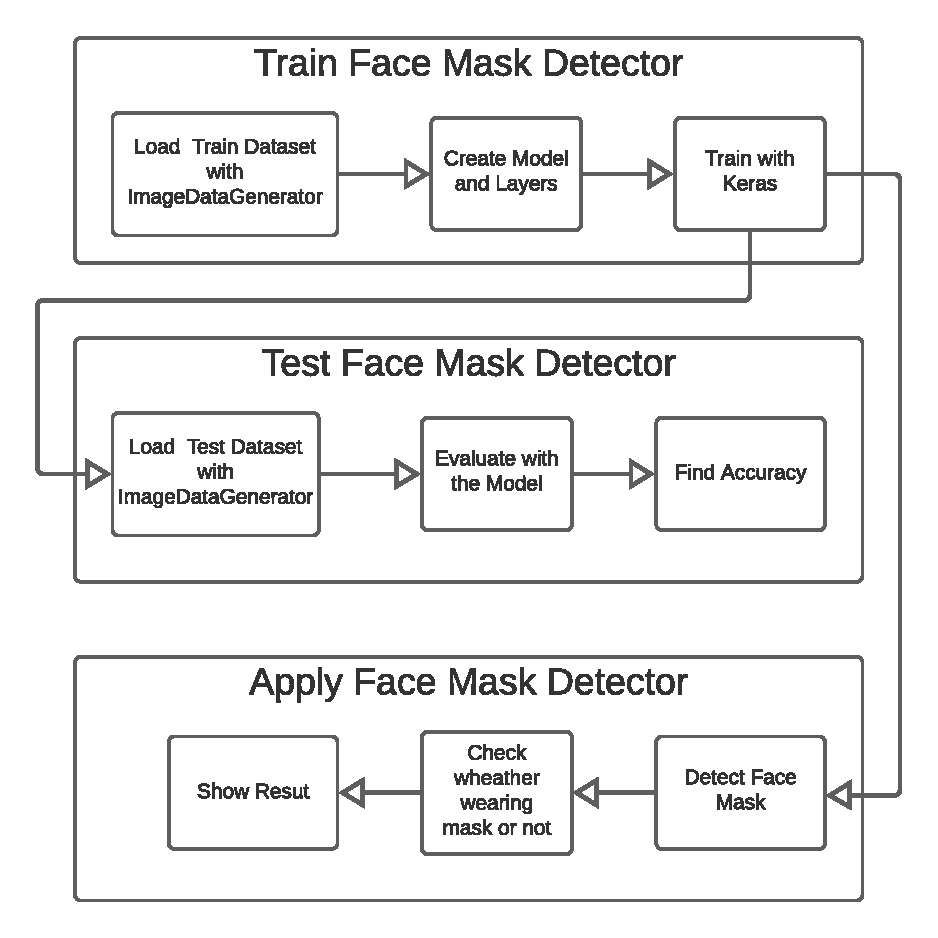
\includegraphics[width=1.0\linewidth]{UpdatedBlockDiagram.pdf}
  \caption{ Architecture of proposed model }
  \label{fig:fig1}
\end{figure}
\end{center}

Here Fig-\ref{fig:fig1} represents our model architecture where, it shows that how our model is going to detect face-mask during COVID-19. First of all we load data-set with the help of TensorFlow,  Keras and ImageDataGenerator and augment the data-set with ImageDataGenerator. We have used a face cropped data-set from Kaggle of about 12,000 images of people with masks and without masks. These images are used in order to train the model that classifies into two categories, which is, faces with masks and faces without masks. These data-sets are then converted into arrays in order 
to create a Deep Learning Model. We used OpenCV to high-level understanging from the digital images. After that we train our model with the augmented train data-set. Once the training is done then we have load the test data-set with the same process and calculated our model accuracy and loss. As our model is done with train and test then we will load the face-mask classifier from the disk and input a particular person's image with the help of tensorFlow, Keras and ImageDataGenerator, after that the classifier will detect whether the person is wearing mask or not. 

\begin{center}
\begin{figure}[htbp]
  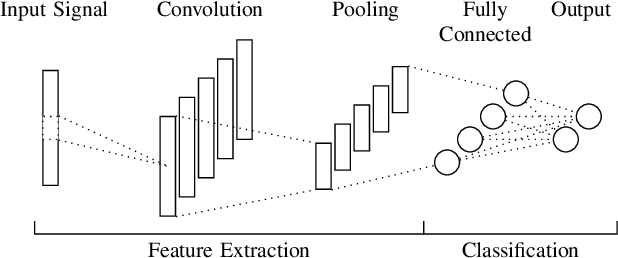
\includegraphics[width=1.0\linewidth]{1-Figure1-1.png}
  \caption{Basic Schematic Diagram for our face-mask detection model }
  \label{fig:fig2}
\end{figure}
\end{center}
\\

Here, Fig- \ref{fig:fig2} shows a basic Schematic Diagram for our face-mask detection model. It is basically a modified version of Convolutional Neural Network(CNN).  CNN plays a significant part in computer vision related examples in recognizing object patterns, with the advantage of  less computation cost and also the ability of spatial extraction. CNN utilizes convolution portions to combine with the primary images in order to remove top-level features. In our proposed model we will use two max-polling layers along with two convolution layers. In the fully connected layer we will have two output layer because there will be two output from our system, which is face with mask and face without mask. We have used 'relu' activation function in the Convolution layer in order to eliminate linearity.

\section{Experimental Results and Analysis }
In this experiment we have built a Convolutional Neural Network classifier along with TensorFlow, Keras, OpenCV and ImageDataGenerator.

\subsection{Data Collection and Pre-Processing}
we collected images from many sources. We used several data-sets from “kaggle” to prepare our own data-set. Finally, we collected about more than 12,000 images for our data-set. In our data-set, we separated the images for testing, training and validation.
\begin{itemize}
  \item Training part has more than 10,000 images 
  \item Validation part has more than 1,000 images 
  \item Testing part has also more than 1,000 images 
\end{itemize}

\begin{center}
\begin{figure}[htbp]
  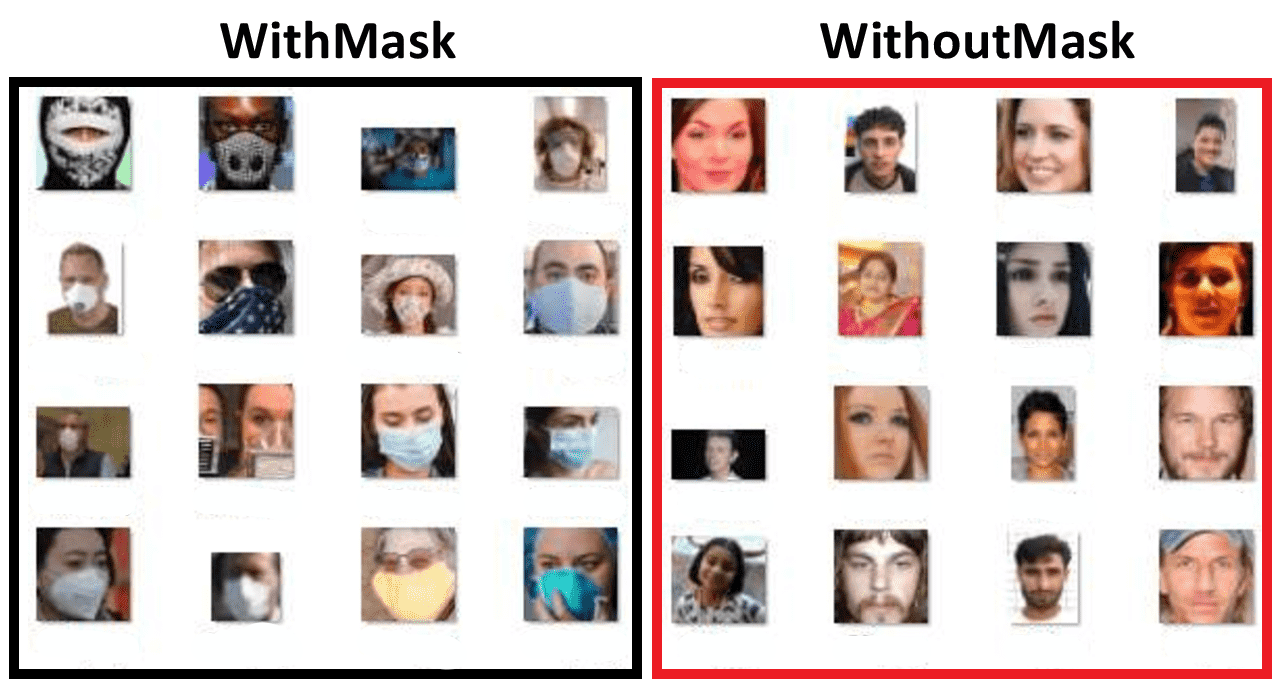
\includegraphics[width=1.0\linewidth]{188500388_1165620213940458_5711695426970840234_n.png}
  \caption{A graph showing a sample data-set, person with mask and without mask}
  \label{fig:fig 9}
\end{figure}
\end{center}

In our data-set each training, testing and validation has two type of data.
\begin{enumerate}
  \item persons face with Face-Mask(fig-\ref{fig:fig 9})
  \item persons face without Face-Mask(fig-\ref{fig:fig 9})
\end{enumerate}

In this project we used “TensorFlow” and “Keras” libraries. Using these two libraries we use “ImageDataGenerator” for processing the data-set. As there are only two image classes in the data-set, we used class\_mode as ‘binary’ and resized the images by (200x200).\\

ImageDataGenerator class provides a quick and easy way to augment the images. It lets us augment the images in real-time while our model is still training. We apply ImageDataGenerator on each training image as it is passed to the model. This saves up on the overhead memory. We also use it to re-scale the images. 

\subsection{Model Training and Testing }
We used a sequential model. We prepared three layers with 64, 32 and 16 features respectively and with ‘relu’ activation function. Then, we flattened our model. After that we added two dense layers and also used 'relu' as activation  function here. In the final layer we used the ‘sigmoid’ activation function as we have only two image classes. In this project, we used more than twelve thousand images for the data-set. Here, we used loss function as ‘binary\_cross-entropy’ and optimizer as ‘adam’. After implementing the described model, we got 98.07\% accuracy in the 10\textsuperscript{th} epoch. 
\begin{center}
\begin{figure}[htbp]
  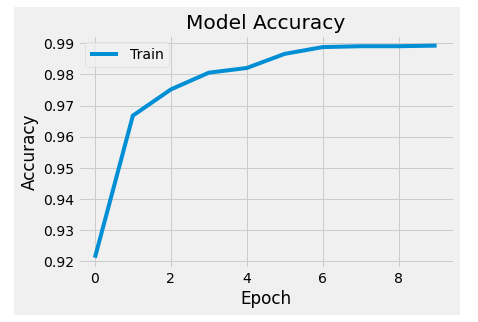
\includegraphics[width=1.0\linewidth]{Accurecy.png}
  \caption{A graph showing the model accuracy}
  \label{fig:fig 3}
\end{figure}
\end{center}
\\

The graph (Fig-\ref{fig:fig 3}) shows that the accuracy of our model is increasing. The maximum accuracy we have got .99 in the last epoch. With that accuracy we can claim that we have got the maximum accuracy among almost all face-mask detector proposed in the past. 
\begin{center}
\begin{figure}[htbp]
  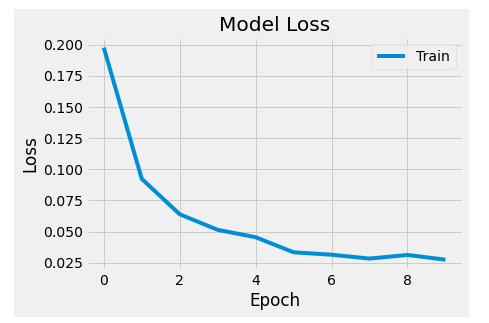
\includegraphics[width=1.0\linewidth]{loss.png}
  \caption{A graph showing the model Loss}
  \label{fig:fig 4}
\end{figure}
\end{center} 
\\

The graph (Fig-\ref{fig:fig 4}) shows that the Loss of our model is decreasing. The minimum loss we have got .0.025 in the last epoch.
\subsection{Real-life Implementation}
Our system can take input of real life images taken from any camera devices of any person. After that it  can find out whether the person in the image is wearing mask or not with the accuracy of 99.07\%.  

\section{Conclusion}
In this research paper we proposed face-mask detection model which can identify a person is wearing face-mask or not. This model can be implement in the crowded area like shopping-mall, educational institute, office, etc to ensure every person is wearing mask in order to prevent the Spreading of coronavirus. In our study we only build a face mask detector (with mask and without mask) but in future the work can be extended to wrong wearing mask detection and social safe distancing detection. In our work we cannot input data from real-time video, so in future the real-time video input feature can be add with this model. 

\bibliographystyle{ieeetr}
\bibliography{Ref}

\end{document}
